\begin{figure}[H]
\centering
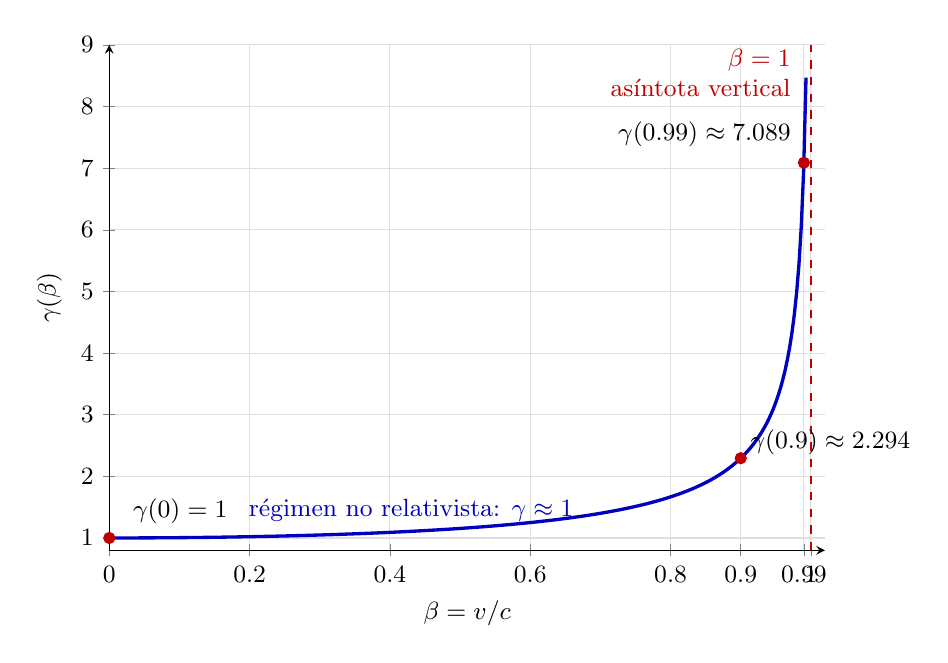
\begin{tikzpicture}
\begin{axis}[
    width=0.88\textwidth,
    height=8.0cm,
    xmin=0,
    xmax=1.02,
    ymin=0.8,
    ymax=9,
    axis lines=left,
    xlabel={$\beta=v/c$},
    ylabel={$\gamma(\beta)$},
    xtick={0,0.2,0.4,0.6,0.8,0.9,0.99,1},
    xticklabels={$0$,$0.2$,$0.4$,$0.6$,$0.8$,$0.9$,$0.99$,$1$},
    ytick={1,2,3,4,5,6,7,8,9},
    grid=major,
    grid style={gray!25},
    tick label style={font=\small},
    label style={font=\small},
    clip=false
]
    \addplot[blue!75!black,very thick,domain=0:0.993,samples=300]
        {1/sqrt(1-x^2)};
    \addplot[red!75!black,thick,dashed]
        coordinates {(1,0.8) (1,9)};

    \addplot[only marks,mark=*,mark size=2pt,red!75!black]
        coordinates {(0,1) (0.9,2.294157) (0.99,7.088812)};

    \node[anchor=south west,font=\small] at (axis cs:0.02,1.08)
        {$\gamma(0)=1$};
    \node[anchor=west,font=\small] at (axis cs:0.9,2.55)
        {$\gamma(0.9)\approx2.294$};
    \node[anchor=east,font=\small] at (axis cs:0.985,7.55)
        {$\gamma(0.99)\approx7.089$};
    \node[red!75!black,anchor=east,font=\small,align=right]
        at (axis cs:0.985,8.55)
        {$\beta=1$\\asíntota vertical};
    \node[blue!75!black,font=\small] at (axis cs:0.43,1.45)
        {régimen no relativista: $\gamma\approx1$};
\end{axis}
\end{tikzpicture}
\caption{Factor de Lorentz $\gamma=(1-\beta^2)^{-1/2}$ en función de $\beta=v/c$. Para velocidades pequeñas, $\gamma$ permanece próximo a uno; cuando $\beta\to1^{-}$, el factor crece sin límite.}
\label{fig:factor-lorentz}
\end{figure}